\input{./../tex_files/preamble_engl}

\usepackage{pstricks,pst-node,pst-tree}
\usepackage{graphicx}


\begin{document}

  \sheet[%
  number=2,
      topic={Graphs },
      %deadline=Deadline: \today,
    ]

\vspace{-1cm}
\noindent\rule{12cm}{0.4pt}

  \exercise[%
  topic = Node colouring 
    ]

%\lstinputlisting{./code/pfadgraph.py}



 \subexercise[%
  topic=Colouring a Graph,
    ]

Find two node colourings for the shown graph.

\begin{figure}[h]
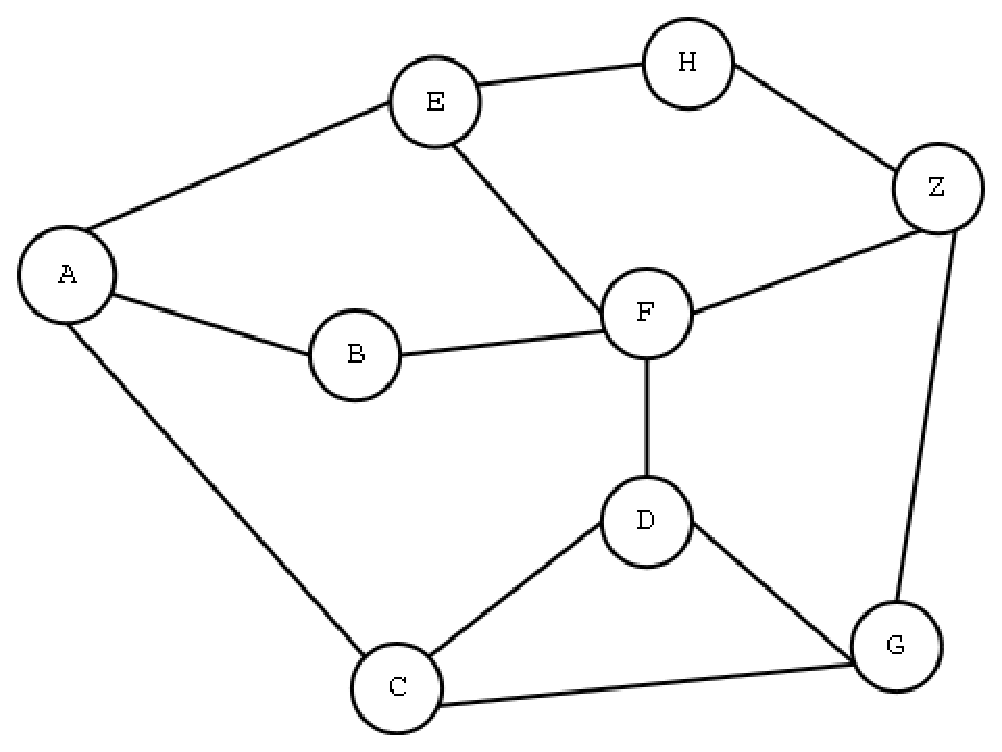
\includegraphics[width=0.4\textwidth]{graph_colouring.eps}
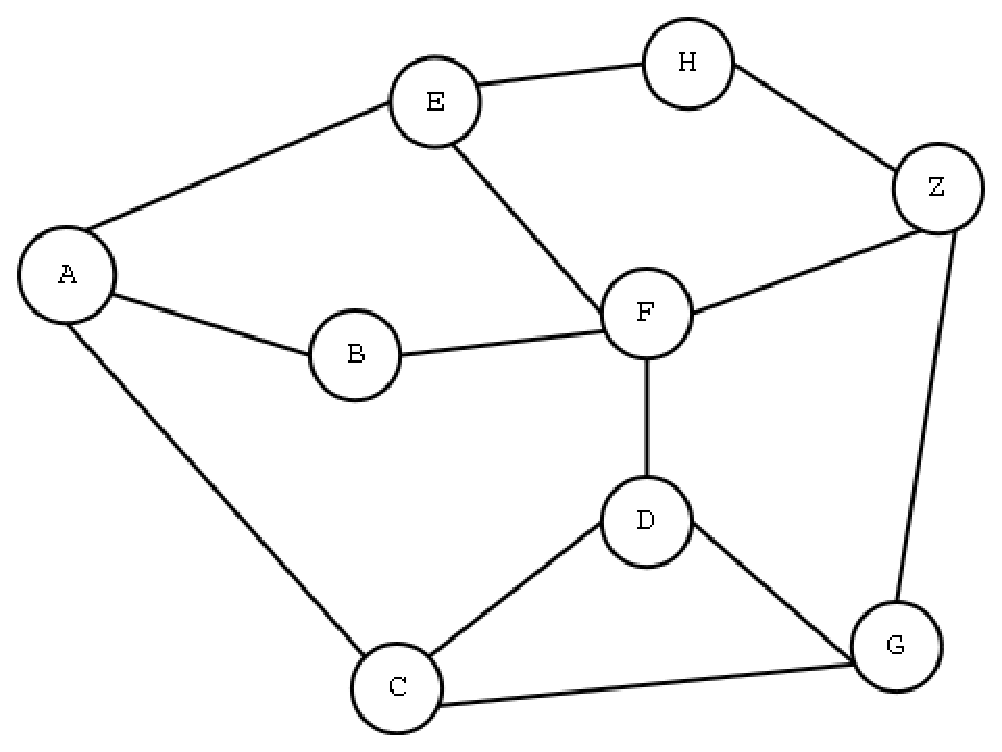
\includegraphics[width=0.4\textwidth]{graph_colouring.eps}
\end{figure}
%\clearpage

How many colours are used for each colouring?

Find a colouring that needs more colours than your first colouring.

What is the maximal number of colours that any colouring can use?

Find the minimal number of colours that a colouring uses. This is also known as \emph{chromatic number} $\chi$.

\subexercise[%
  topic=Chromatic Number of Graph Models,
    ]
		\label{subseq:graphen}
		
Find the chromatic number $\chi$ of the following graphs in depency of the number $n$ of nodes:

\begin{enumerate}
\item null graph $N_n$
\item path graph $P_n$
\item cycle graph $C_n$
\item complete graph $K_n$
\item complete bipartite graph $K_{n/2,n/2}$
\end{enumerate}

\subexercise[%
  topic=Chromatic Number,
    ]
 
 Find two nonisomorph graphs with $n=5$ nodes and the chromatic number $\chi=3$.   
 

\subexercise[%
  topic=Zoo director,
    ]
  
  A zoo director wants to host the following five animals in as few
  cages as possible: Eagle, snake, mouse, lion, and goat. Find the
  necessary number of cages if the following animals are not allowed in
  the same cage: eagle \& snake, snake \& mouse, lion \& goat.
  

\subexercise[%
  topic=Petersen Graph,
    ]
    
In Figure~\ref{petersen} you can see the so called \emph{Petersen graph}. Find its chromatic number $\chi$. Sketch a  $\chi$-colouring on it.    
    
\begin{figure}[h]
    \centering
    \includegraphics[width=0.4\textwidth]{petersen_graph.eps}
    \caption{\label{petersen} The Petersen graph.}

%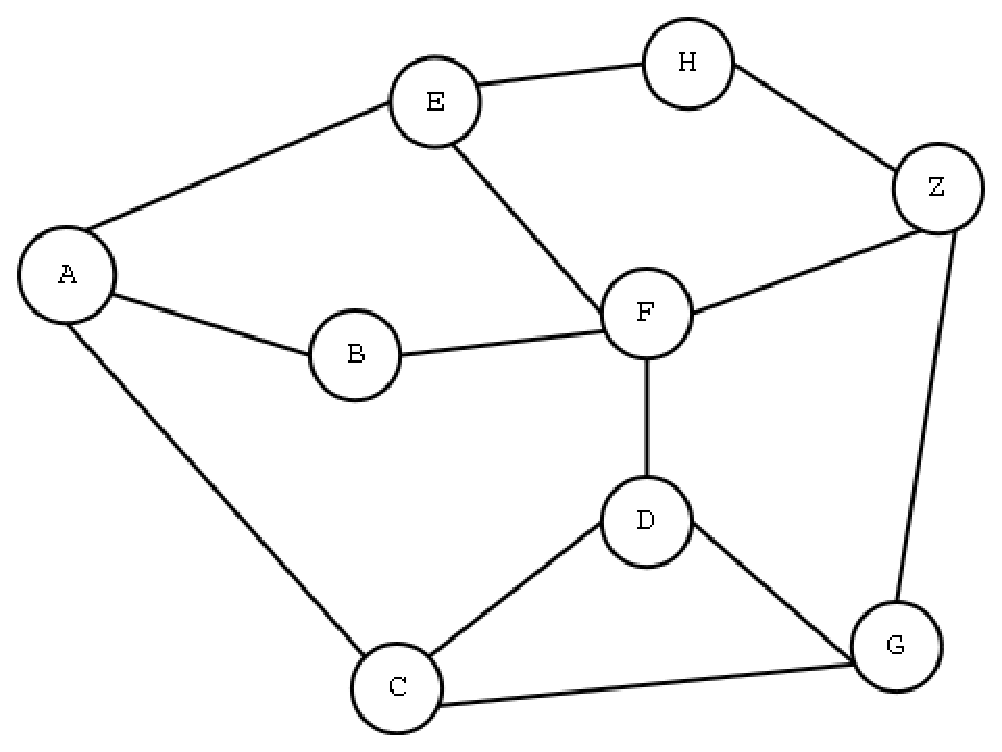
\includegraphics[width=0.4\textwidth]{graph_colouring.eps}
\end{figure}



\subexercise[%
  topic=Graphs of Different Size but Same Chromatic Number
    ]
		
	Find two graphs $G$ and $H$ such that they have the same number $n$ of nodes and $m$ of edges but $\chi (G)> \chi (H)$.



\subexercise[%
  topic=An upper bound for the chromatic number,
    ]
    
Let $G$ be a graph with $n$ nodes and {\bf not} the complete graph
$K_n$. Show that $\chi (G) < n$. \emph{Hint: It might be useful to first
    prove the following lemma: Shall $c(V)$ be a proper colouring of the graph $G=(V,E)$. 
    Then $c(V)$ is also a proper colouring of the graph $G'=(V,E')$ with $E'\subset E$ }
    


\exercise[%
  topic = Graph isomorphism 
    ]
		
		\subexercise[%
  topic=Check the isomorphism between graphs,
    ]
		
		
Which of the graphs shown below are isomorph? For those of them that are isomorph find the isomorphism function. For the other find a graph theoretical metric that distinguishes them such that they can not be isomorph.		
		
\begin{figure}[h]
    \centering
    \includegraphics[width=0.9\textwidth]{isomorphism_cut.pdf}
    \caption{\label{isomorphismus} Which of these graphs are isomorph?}
\end{figure}

\subexercise[%
  topic=2-regular Graphs,
    ]

The set of all 2-regular graphs can also be called the \emph{disjoint union of all cycle graphs}. Find different 2-regular graphs with $n=10$ nodes. Prove that the graphs are not isomorph.
    
    
\clearpage 
\exercise[%
  topic =Edge Colouring 
    ]

\subexercise[%
  topic=Edge Colouring of a Graph,
    ]

Find a proper edge colouring for the graph shown below. The colouring
should use exactly $\Delta$ colour, where $\Delta$ is the graph's maximal
degree. What is the chromatic index $\chi'$ of the graph?

\begin{figure}[h]
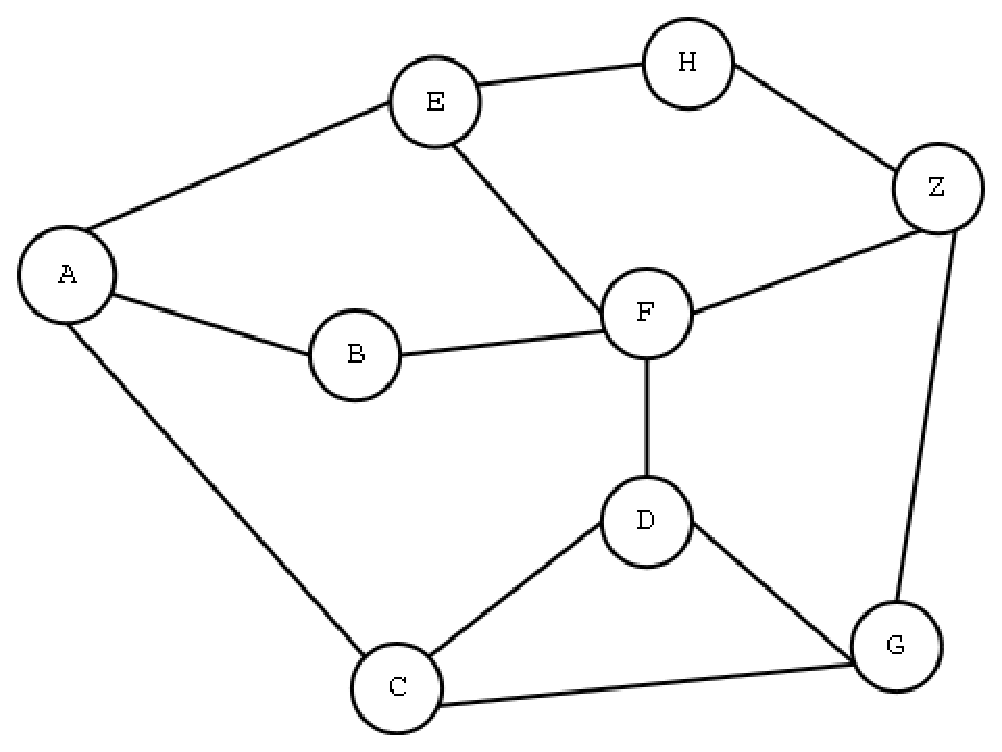
\includegraphics[width=0.4\textwidth]{graph_colouring.eps}
%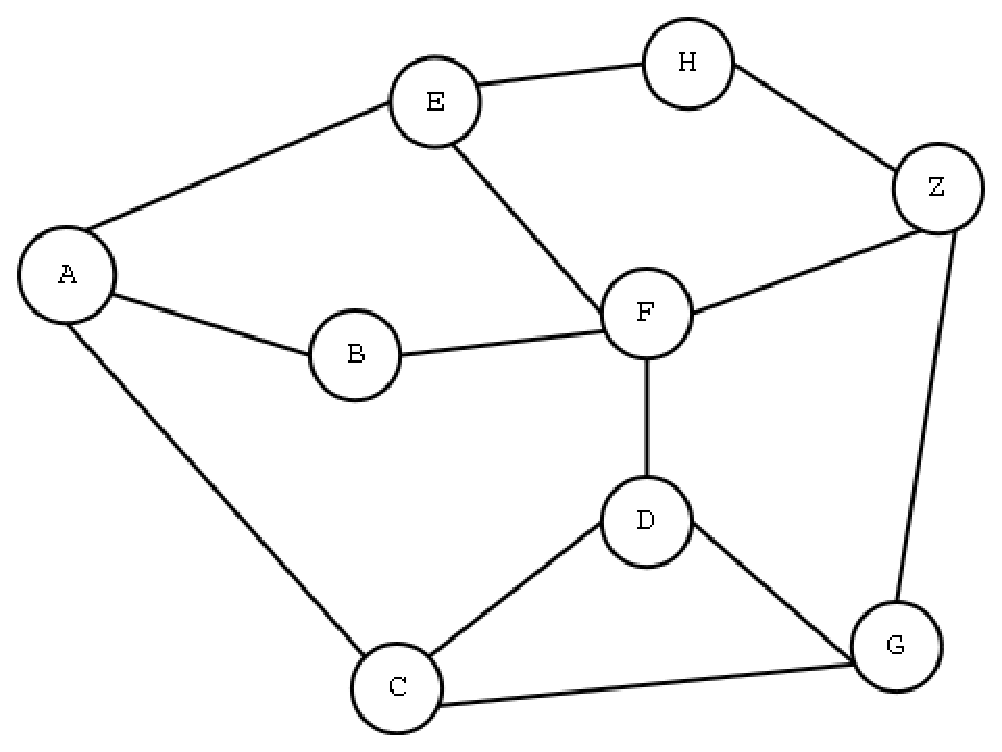
\includegraphics[width=0.4\textwidth]{graph_colouring.eps}
\end{figure}

\subexercise[%
  topic=Edge colouring of Graph Models,
    ]

Find the  chromatic index  $\chi'$ in dependence of the number $n$ of nodes of the following graphs:   

\begin{enumerate}
\item path graph $P_n$
\item cycle graph $C_n$
\item complete graph $K_n$ (tricky, potentially skip)
\end{enumerate}

Compare for these graphs the chromatic index  $\chi'$  with the maximal degree $\Delta$.

\exercise[%
  topic = Coding the Greedy Colouring
    ]

We want to program the \emph{greedy node colouring algorithm} and use it on different networks.

\subexercise[%
  topic=Greedy Colouring,
    ]
    
    
    Create a function that takes as input the adjacency matrix $A$ of a
    graph and an ordering of the nodes and returns a proper colouring of
    the graph by using the greedy colouring algorithm. 
    

\subexercise[%
  topic=Greedy Colouring of Graph Models,
    ]
    
Use the greedy colouring algorithm on the graphs from Subexercise~\ref{subseq:graphen} with a chosen size of $n=10$. Use different random orderings of the nodes. Compare the results for different realisations amongst each other and with the analytical formulas you derived for the chromatic number $\chi$.
    
   
		
		
		\subexercise[%
  topic=Time Complexity of the Greedy Colouring Algorithm,
    ]

We want to use the greedy colouring algorithm on random graphs of size $n$. To find the chromatic number of a graph with certainty we have to check all possible node orderings. 

How many node orderings exist in dependency of the number $n$ of nodes? 

Using this insights compute numerically the time complexity of the greedy algorithm to find the chromatic number $\chi$ of a graph with size $n$.


\exercise[%
  topic=Placing Animals in Cages ,
    ]



Load the network from the file  {\tt everglades\textunderscore
    adjazenz.txt}. It represents the food chain of animals in the
Everglades national park in Florida. The animals are connected if they
are in a predator--prey relationship. A zoo wants to place all $63$
animals in as few cages as possible. To avoid them killing each other no
pair of animals is allowed to be kept in the cage if one potentially
preys on the other. The file  {\tt everglades\textunderscore namen.txt}
gives the names of the animals.

Formulate the problem as a graph theoretical one and solve it
numerically. For this use the greedy colouring algorithm on random
orders of the nodes. Is it possible to check all orderings? Illustrate
the graph and show the cage assignment that uses the least number of
cages.

\exercise[%
  topic=Chromatic Polynom,
    ]

Research the definition of the \emph{chromatic polynom}, as well as, the definition of a \emph{tree} graph. Then prove that the chromatic polynom of the empty graph is $\chi_{N_n}(t) =t$, the one of the complete graph is $\chi_{K_n}(t) =t^n$, and of a tree is given by
\begin{align}
\chi_{G(t)} = t(t-1)^{n-1}\,.
\end{align}

 


	
\end{document}
